\ProvidesFile{titlepage.tex}[2003/07/01 HighTec Vorlage]
%%%%%%%%%%%% titlepage %%%%%%%%%%%%%%%%%%%%%%%%%%%%%%%%%%%%%%%%%%%
\newcommand{\clearemptydoublepage}{\newpage{\pagestyle{empty}\cleardoublepage}}
\pagenumbering{roman}
\makeatletter
\@ifundefined{htmlmode}{%
    \begin{titlepage}
    \begin{flushleft}
    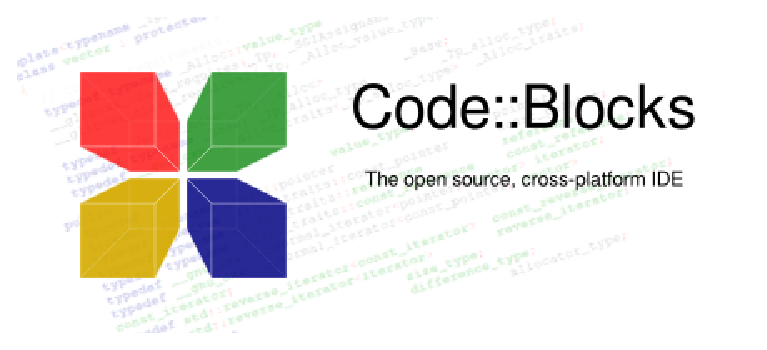
\includegraphics[width=\columnwidth]{mystyles/cb_splash}
    \vfill
    \makeatletter
    \@ifundefined{Subtitle}{%
        {\Huge\textbf{\Subject}\\ [2ex] \Title\\ [2ex] \large{Version \DocVersion}\\ [2ex]}
    }{%
        {\Huge\textbf{\Subject}\\ [2ex] \Title\\ \Subtitle\\ [2ex] \large{Version \DocVersion}\\ [2ex]}
    }
    \makeatother
    \vfill
    Thanks to the \codeblocks team:\\

    Anders F. Bj\"{o}rklund (afb), Biplab Kumar Modak (biplab), Bartomiej wiecki (byo),
    Paul A. Jimenez (ceniza), Koa Chong Gee (cyberkoa), Daniel Orb (daniel2000), Lieven de Cock (killerbot), Yiannis Mandravellos (mandrav), Mispunt (mispunt), Martin Halle (mortenmacfly), Jens Lody (jens), Jerome Antoine (dje), Damien Moore (dmoore),
    Pecan Heber (pecan), Ricardo Garcia (rickg22), Thomas Denk (thomasdenk), tiwag (tiwag), stahta01 (stahta01), Teodor Petrov (oBFusCATed), BlueHazzard (BlueHazzard), Andrew Cottrell (AndrewCot), Miguel Gimenez (wh11204) 

    And many other contributors...

    Original manual in English and in German (V1.x) by Mario Cupelli (mariocup)\\
    Translation in French (v1.x), corrections and additions for version 2 by Gerard Durand (gd\_on).\\
    Some paragraphs are directly imported from \codeblocks WiKi. Don't hesitate to visit \url{https://wiki.codeblocks.org/index.php/Main_Page}, informations are perhaps more up to date.\\

    Permission is granted to copy, distribute and/or modify this document under the terms of the GNU Free Documentation License, Version 1.2 or any later version published by the Free Software Foundation.

    User Manual updated in june 2023
    \end{flushleft}
    \end{titlepage}
    \pagestyle{headings}
%%%%%%%%%%%% Table of contents %%%%%%%%%%%%%%%%%%%%%%%%%%%%%%%%%%%%%%%%%%%
% This ifthenelse is desactivated, because it has problems with recent Miktex versions (22.10), though it was OK with a previous one (22.03).
% More, it's only used when shortdocu is false, which is not the standard case for C::B documentation.
%    \ifthenelse{\boolean{shortdocu}}{}{
%%        \tableofcontents
%        \ifthenelse{\boolean{figreg}}{\listoffigures}{}
%        \ifthenelse{\boolean{tabreg}}{\listoftables}{}
%    }
%    \clearemptydoublepage \pagestyle{headings}
    \pagenumbering{arabic}
}{%
    \begin{titlepage}
        \@ifundefined{Subtitle}{%
            \Huge\textbf{{\Subject} {\Title}}\\
        }{
            \Huge\textbf{{\Subject} {\Title} {\Subtitle}}\\
        }
        \large{Version \DocVersion}
    \end{titlepage}
    \clearemptydoublepage \pagestyle{headings}
    %\tableofcontents
    \clearemptydoublepage \pagenumbering{arabic}
    \pagenumbering{arabic}
}
\makeatother
